\documentclass[11pt]{article}
\usepackage{amsmath,amssymb,amsthm}
\usepackage{booktabs}
\usepackage{graphicx}
\usepackage{xcolor}
\usepackage{microtype}
\usepackage[margin=1in]{geometry}
\usepackage{algorithm}
\usepackage[colorlinks=true,linkcolor=blue!55!black,citecolor=blue!55!black,urlcolor=blue!55!black]{hyperref}

\newtheorem{theorem}{Theorem}
\newtheorem{proposition}[theorem]{Proposition}
\newtheorem{lemma}[theorem]{Lemma}
\newtheorem{corollary}[theorem]{Corollary}
\theoremstyle{definition}
\newtheorem{definition}[theorem]{Definition}
\newtheorem{assumption}[theorem]{Assumption}
\newtheorem{example}[theorem]{Example}
\theoremstyle{remark}
\newtheorem{remark}[theorem]{Remark}

\newcommand{\R}{\mathbb{R}}
\newcommand{\norm}[1]{\lVert #1 \rVert}
\newcommand{\abs}[1]{\lvert #1 \rvert}
\newcommand{\diam}{\operatorname{diam}}
\newcommand{\diag}{\operatorname{diag}}
\newcommand{\grad}{\nabla}
\newcommand{\betamax}{\beta_{\max}}

\title{\bfseries Certified Equilibrium Propagation in\\ Non-Conservative Multistable Systems:\\[3pt]
Exact Gradient Conditions and Finite Perturbation Guarantees}
\author{Sheng Cheng\\ \small Hefei Jiuzhai Big Data Technology Co., Ltd.\\ \small \texttt{github.com/hf-jz}}
\date{October 2026}

\begin{document}
\maketitle

\begin{abstract}
\noindent
Equilibrium propagation (EP) computes a learning signal from the response of a physical or
simulated dynamical system to a weak perturbation of its stationary state. The classical
guarantee rests on an energy function, which forces the state Jacobian to be symmetric. Recent
work has removed the symmetry requirement, and finite-nudge exactness has been established for
contrastive free-energy objectives in thermal ensembles. What remains open is computational:
a finite-precision procedure returns two numerical states, and no criterion determines whether
the gradient read from them meets a stated tolerance, or whether the states belong to the
intended equilibrium branch of a multistable system. We address that
question analytically and numerically. First, we isolate the exact gradient conditions for
general smooth non-conservative equilibrium systems and show how the equilibrium sensitivity
$A^{-1}q$ differs from the adjoint quantity $A^{-\top}q$ the parameter gradient requires, a
distinction that vanishes in the conservative case and that explains the residual bias of
standard vector-field EP. Second, we derive a finite-perturbation error budget with computable
constants: a second-order contrast bias, a solver term that grows as $1/\betamax$, a finite-time
integration term, and a rounding term. Third, we convert the budget into a fail-closed
certification algorithm built on interval Krawczyk operators over exact rational arithmetic,
which certifies branch existence and uniqueness uniformly over a parameter interval, encloses
the centred finite difference, and accepts or rejects an update against a prescribed tolerance.
On an exactly solvable two-dimensional non-conservative system with two stable equilibria and a
saddle, both stable branches and both perturbation endpoints are certified with a preconditioned
contraction factor of $2249/13600$; the controller accepts $\betamax = 0.005$ with a worst-branch
gradient error bound of $7.53\times10^{-6}$ at tolerance $10^{-5}$ and rejects every larger tested
candidate, including a deliberately broad box that spans all three equilibria. On a three-state
non-normal benchmark the certified residual run bounds the gradient error by
$4.39\times10^{-4}$ at tolerance $5\times10^{-4}$ while the observed error is
$1.08\times10^{-5}$. We also quantify why finite-time guarantees must not be read off the
spectrum: systems with fixed eigenvalues can amplify the adjoint response by a factor of $15.5$,
and the corresponding Lyapunov envelope, while valid, exceeds the observed error by four orders of
magnitude. All numbers in this paper are produced by the accompanying package in
under a minute.

\vspace{6pt}
\noindent\textbf{Keywords:} equilibrium propagation; non-conservative dynamics; implicit
gradient; finite perturbation; interval arithmetic; Krawczyk operator; certification;
multistable systems.
\end{abstract}

\tableofcontents

\section{Introduction}

Equilibrium propagation (EP) trains a dynamical system by comparing two of its stationary
states \cite{scellier2017}. In the free phase the system relaxes under the input alone; in the
nudged phase the loss contributes a weak force that pushes the state toward a target. The
difference between the two states, read through local quantities, estimates the gradient of the
loss with respect to the parameters. Because the two phases use the same dynamics, EP is a
candidate learning rule for analog, neuromorphic and physical substrates, where a distinct
backward pass is unavailable \cite{kendall2020,yi2023,hoier2023}.

The classical derivation assumes an energy function $E$ with $\dot z = -\grad_z E$. Then the
state Jacobian at a stationary point is symmetric, the state response and the adjoint response
coincide, and the two-phase contrast reproduces the gradient. Symmetric coupling is rarely
available in hardware: memristive crossbars, optical and mechanical networks, and
feedforward architectures all realize non-reciprocal interactions. Two lines of work address
this. The vector-field generalization replaces the energy by an arbitrary force field and keeps
the two-phase rule, at the cost of a bias that grows with the antisymmetric part of the Jacobian
\cite{scellier2018,laborieux2024}. More recently, exact-gradient algorithms for non-conservative
systems have been proposed: an augmented learning phase whose Jacobian is corrected by the
antisymmetric part of the free-equilibrium Jacobian, and a variational construction on a doubled
state space \cite{scurria2026}. In parallel, EP has been placed on a statistical foundation.
For real-valued Gibbs ensembles the contrast between the nudged and free Helmholtz free energies
has an exact gradient at every finite temperature and every finite nudging strength, so that the
finite-nudge bias of the deterministic rule is a consequence of taking the zero-temperature limit
rather than of contrastive learning itself \cite{litman2026}. Quantum and thermal versions of the
same response identities are developed in \cite{massar2025}.

These results settle what the algorithm computes in exact arithmetic, to first order, or in the
thermodynamic limit. They do not address the status of the numerical output of a run, which is
floating-point states obtained from a root finder or an ODE integrator; the reported gradient is
a quotient by a small number; and in a multistable system the two states may belong to different
equilibrium branches. A small residual at the returned states is not a correctness argument:
it bounds how well the iterate solves the equations the practitioner wrote down, not the distance
to the true stationary state, and it says nothing about branch identity. The question we address
is therefore the following.

\begin{quote}
Given a smooth non-conservative equilibrium system with a regular local equilibrium, a
finite nudging strength, and a target tolerance, when may the EP gradient estimate computed from
numerical stationary states be declared trustworthy, and how much error must be attributed to it?
\end{quote}

Answering it requires three objects that are usually kept apart: the exact gradient identity, the
finite-perturbation error budget, and a branch-aware numerical certificate. This paper joins
them, and verifies the join on systems whose exact answers are known in rational arithmetic.

\subsection{Contributions}

\begin{enumerate}
\item \textbf{Exact gradient conditions and the sensitivity-adjoint dichotomy.} For
$\dot z = F(z,\theta)$ with a regular equilibrium we give the implicit gradient
$\grad_\theta L = \partial_\theta C - B^{\top}A^{-\top}q$ (Theorem~\ref{thm:implicit}), the
exactness condition for standard vector-field EP as a single bias term
$B^{\top}(A^{-1}-A^{-\top})q$ together with a task-restricted exactness criterion
(Theorem~\ref{thm:vf}), and the observation that the centred contrast of the \emph{uncorrected}
nudged system measures the equilibrium sensitivity $A^{-1}q$ rather than the adjoint
$A^{-\top}q$ (Proposition~\ref{prop:sens}). The two coincide only when $A = A^{\top}$, which is
why conservative EP cannot see the distinction and why non-conservative EP must.
\item \textbf{Finite-perturbation budget with computable constants.} We prove that the centred
contrast of the antisymmetry-corrected learning phase is second order in the nudging strength
(Theorem~\ref{thm:secondorder}), identify the resulting trade-off between the $O(\betamax^2)$
contrast bias and the $O(1/\betamax)$ amplification of state error, give the corresponding
optimal scale $\beta^\ast = (d/(2a))^{1/3}$, and assemble the budget
$E_{\mathrm{total}} \le E_{\beta} + E_z + E_t + E_{\mathrm{fp}}$ with every constant obtained by
interval evaluation rather than fitted.
\item \textbf{Branch-aware certification.} We certify existence and uniqueness of the free
equilibrium, of both perturbation endpoints, and of the whole branch tube uniformly over a
parameter interval, using exact rational Krawczyk operators, together with a Hurwitz test that is
uniform on the tube; the centred finite difference is enclosed by interval arithmetic and
compared with the exact rational gradient. The resulting algorithm is fail-closed: it either
returns an interval containing the gradient with a certified error bound, or it refuses.
\item \textbf{Verified benchmarks with rejection paths.} A two-dimensional non-conservative
system with two stable equilibria and a saddle is certified end to end in exact rational
arithmetic, including the rejection of a wide box that contains all three equilibria and the
rejection of nudging strengths whose bound exceeds tolerance. A three-state non-normal benchmark
carries a certified residual run, an adaptive controller whose selected settings are cross-checked
against a high-accuracy integrator, and a bounded-state-noise stress test.
\end{enumerate}

\subsection{Scope}

We establish certified gradient conditions for a broad class of smooth non-conservative
equilibrium systems with regular isolated equilibria ($F \in C^3$, $\sigma_{\min}(A) > 0$). We do
not claim convergence of arbitrary nonlinear dynamics of arbitrary stability type, we do not
claim global optimality of the selected nudging strength, and we do not claim that a certificate
transfers to systems whose coefficients are uncertain or whose trajectories are only partially
observed. The certified statements in Section~\ref{sec:results} are statements about the
explicitly defined benchmarks; their conclusions are intervals that contain the exact rational
answer, not performance claims about neural networks. We do not propose a new EP update rule: the
antisymmetry-corrected phase and the doubled-state construction are prior work
\cite{scurria2026,hoier2023}, and we use them as the objects of certification. The unit of
certification is one gradient estimate, at one parameter point, on one certified branch: nothing
here certifies the training trajectory that later consumes the estimate.

\section{Related work}

\paragraph{Equilibrium propagation and energy-based models.}
EP was introduced for continuous Hopfield energies and proved to perform gradient descent on a
squared-error objective \cite{scellier2017,hopfield1984}. Its second phase is equal, at every
instant, to the error propagation of recurrent backpropagation \cite{ernoult2019,pineda1987}.
Contrastive Hebbian learning is the historical relative \cite{movellan1991}; the equivalence of
EP and contrastive rules for energy-based models is part of the original derivation.

\paragraph{Beyond symmetric coupling.}
The vector-field generalization removes the energy assumption and with it the symmetry of the
Jacobian \cite{scellier2018}. The two sources of bias, finite nudge and Jacobian asymmetry, were
separated in \cite{laborieux2024}, where a homeostatic penalty on the antisymmetric part of the
Jacobian substantially improves performance without enforcing weight symmetry, and where exact
derivatives are recovered in complex-differentiable networks by a Cauchy integral. An exact
gradient for general non-conservative systems was obtained in \cite{scurria2026} by adding a
learning-phase force proportional to the antisymmetric part of the free-equilibrium Jacobian,
equivalently by a variational construction on a doubled state space; dual propagation is the
related compartmental construction \cite{hoier2023}. Our certification applies to these
constructions.

\paragraph{Finite nudging.}
Finite nudging is not a defect per se. For Gibbs ensembles the two-phase contrast is the exact
gradient of a free-energy difference at any finite nudging strength and temperature, and a
low-temperature limit recovers the deterministic rule \cite{litman2026}; the quantum and thermal
cases are treated in \cite{massar2025}. The quantity that remains to be controlled in the
deterministic setting is therefore the distance between the deterministic finite-nudge contrast
and the exact gradient, which is the object of Theorem~\ref{thm:secondorder}.

\paragraph{Implicit differentiation and stationary-state models.}
Gradients of a stationary state with respect to parameters are given by the implicit function
theorem; deep equilibrium models make the same construction computational
\cite{bai2019,laborieux2024}. Implicit differentiation provides the gradient analytically; the
question we study is when a \emph{dynamical} perturbation procedure realizes it with a finite
error guarantee, which is a stricter requirement than differentiability.

\paragraph{Verified numerics.}
The Krawczyk operator is a classical inclusion test for systems of equations
\cite{krawczyk1969,neumaier1990}; verification methods based on floating-point interval
arithmetic can produce rigorous inclusions at moderate cost \cite{rump2010}. We use them here
over exact rational arithmetic rather than directed rounding, so that the accepted conclusions
carry no rounding model beyond the explicitly converted binary rationals of the candidate states.

\paragraph{Non-normality.}
When the state Jacobian is far from symmetric, the spectrum does not control transient
behaviour; the relevant objects are the numerical range, the semigroup norm and the
pseudospectrum \cite{trefethen2005,higham2008}. Section~\ref{sec:nonnormal} shows that this is
not a technicality for EP: the finite-time adjoint tail is governed by the semigroup, not by the
spectral abscissa.

\section{Setting and notation}\label{sec:setting}

\subsection{Parameterized equilibrium systems}

Let $z \in \R^n$ denote the state and $\theta \in \R^p$ the learnable parameters of a
dynamical system
\begin{equation}
\dot z = F(z,\theta), \qquad F \in C^3(\R^n \times \R^p; \R^n),
\label{eq:dynamics}
\end{equation}
whose trajectories converge to a stationary state. No scalar potential is assumed: $F$ need not
equal $-\grad_z E$ for any $E$, and the Jacobian
\begin{equation}
A = D_z F(z^\star,\theta), \qquad B = D_\theta F(z^\star,\theta)
\label{eq:AB}
\end{equation}
at the free equilibrium $z^\star$ need not be symmetric. Let $C$ be a differentiable loss and
\begin{equation}
q = \grad_z C(z^\star,\theta)
\label{eq:q}
\end{equation}
its state gradient at the free equilibrium; $C$ may depend explicitly on $\theta$, in which case
$\partial_\theta C$ denotes that partial derivative.

\begin{assumption}[Regular local equilibrium]\label{ass:regular}
$F(z^\star,\theta) = 0$ and $\det A \neq 0$, so that by the implicit function theorem a unique
local branch $z^\star(\theta)$ of equilibria passes through $(z^\star,\theta)$.
\end{assumption}

Assumption~\ref{ass:regular} is the only regularity requirement behind the gradient identities
of Section~\ref{sec:exact}. Two further conditions appear later: a uniform contraction bound on a
neighbourhood of the branch wherever we certify numerically, and a bounded certified parameter
domain wherever the perturbation strength is treated as an interval.

\subsection{Three learning-phase dynamics}

The three dynamics below are the objects the paper distinguishes. All three read a gradient
estimate out of a centred contrast of two stationary states,
\begin{equation}
\widehat{g}_\beta = B^{\top}\frac{z^{+\beta} - z^{-\beta}}{2\beta},
\label{eq:contrast}
\end{equation}
and they differ only in the equations that define those states.

\paragraph{(i) Standard vector-field EP (uncorrected).}
\begin{equation}
F(z^{\pm\beta},\theta) \mp \beta \grad_z C(z^{\pm\beta},\theta) = 0 .
\label{eq:vf}
\end{equation}

\paragraph{(ii) Antisymmetry-corrected learning phase (AsymEP).}
With $A_{\mathrm a} = \tfrac12 (A - A^{\top})$ evaluated at the free equilibrium and held fixed
during the learning phase,
\begin{equation}
F(z^{\pm\beta},\theta) \mp \beta \grad_z C(z^{\pm\beta},\theta) - 2A_{\mathrm a}\bigl(z^{\pm\beta} - z^\star\bigr) = 0 .
\label{eq:asym}
\end{equation}

\paragraph{(iii) Doubled-state system (Dyadic EP).}
With midpoint $m = \tfrac12 (z + z')$ and difference $d = z - z'$, the stationary state of the
doubled system satisfies
\begin{equation}
F(m,\theta) = 0, \qquad A(m,\theta)^{\top} d = \beta\, \grad_m C(m,\theta),
\label{eq:dyadic}
\end{equation}
where $A(m,\theta) = D_m F(m,\theta)$ \cite{scurria2026}. Equation~\eqref{eq:dyadic} uses the
centred contrast \eqref{eq:contrast} in the form $\widehat{g}_\beta = B(m,\theta)^{\top} d/\beta$.

\subsection{Three levels of evidence}

Throughout, we separate three levels that are often conflated.
\begin{itemize}
\item \textbf{Analytic}: an identity, inequality or criterion proved for the model as written,
without reference to a computation.
\item \textbf{Floating-point diagnostic}: numbers produced by a numerical solver, informative
about behaviour but not a proof of anything, in particular not of the distance to an exact root.
\item \textbf{Certificate}: an enclosure produced by interval arithmetic from the exact rational
conversion of the candidate states, whose acceptance is a mathematical statement about the model.
A certificate can fail; failure is reported, never repaired by tightening a tolerance after the
fact.
\end{itemize}

\section{Exact gradient conditions}\label{sec:exact}

\subsection{The implicit gradient}

\begin{theorem}[Equilibrium sensitivity and implicit gradient]\label{thm:implicit}
Let Assumption~\ref{ass:regular} hold, let $L(\theta) = C(z^\star(\theta),\theta)$ be the
objective evaluated at the equilibrium branch, and let $A$, $B$, $q$ be as in
\eqref{eq:AB}--\eqref{eq:q}. Then
\begin{equation}
D_\theta z^\star = -A^{-1}B,
\qquad
\boxed{\ \grad_\theta L = \partial_\theta C - B^{\top} A^{-\top} q\ }
\label{eq:grad}
\end{equation}
and, when $C$ does not depend explicitly on $\theta$, the true negative gradient reads
$d^\star = B^{\top}A^{-\top} q$.
\end{theorem}

The proof is in Appendix~\ref{app:proofs}. Equation~\eqref{eq:grad} requires nothing beyond a
regular local equilibrium; it applies to dissipative, non-reciprocal and feedforward force fields
alike. It is also the exact target that any EP procedure has to approximate, and every error
bound below is measured against it.

\subsection{Sensitivity is not the gradient}

\begin{proposition}[Sensitivity and adjoint]\label{prop:sens}
Define the equilibrium sensitivity $s$ and the adjoint $\lambda$ by
\begin{equation}
A s = q, \qquad A^{\top} \lambda = q,
\label{eq:sens}
\end{equation}
that is $s = A^{-1}q$ and $\lambda = A^{-\top}q$. The centred contrast of the uncorrected nudged
system \eqref{eq:vf} satisfies
\begin{equation}
\frac{z^{+\beta} - z^{-\beta}}{2\beta} = s + O(\beta^2),
\end{equation}
while the parameter gradient of Theorem~\ref{thm:implicit} is read through $\lambda$. If
$A = A^{\top}$ then $s = \lambda$ and the two notions coincide.
\end{proposition}

Proposition~\ref{prop:sens} is the reason non-conservative systems need a corrected learning
phase. It also identifies a failure mode of the numerical practice: a two-phase run with small
residuals may still yield an incorrect direction whenever $A$ is not symmetric, and the
discrepancy is not small unless $q$ happens to lie in a subspace on which the two responses agree. Table~\ref{tab:levels} records this on the benchmark of
Section~\ref{sec:multistable}: the two quantities are $-0.3235294118$ and $-0.3627450980$,
a relative difference of $12\%$.

\subsection{Bias of the uncorrected vector-field rule}

\begin{theorem}[Vector-field EP bias]\label{thm:vf}
Let the uncorrected states solve \eqref{eq:vf} and let $\widehat{g}_\beta$ be the contrast
\eqref{eq:contrast}. Then the infinitesimal contrast is $B^{\top}A^{-1}q$, so that against the
true negative gradient $B^{\top}A^{-\top}q$ the bias is
\begin{equation}
\boxed{\ e_{\mathrm{VF}} = B^{\top}\bigl(A^{-1} - A^{-\top}\bigr) q\ }
\label{eq:vf-bias}
\end{equation}
and the rule is exact at the given parameter point for the given task if and only if
$B^{\top}(A^{-1}-A^{-\top})q = 0$. If the loss gradients range over a subspace $S \subset \R^n$,
exactness for every task in $S$ holds if and only if
\begin{equation}
B^{\top}\bigl(A^{-1} - A^{-\top}\bigr) S = \{0\}.
\label{eq:vf-subspace}
\end{equation}
\end{theorem}

\begin{example}[Task-restricted exactness without symmetry]\label{ex:restricted}
Take
\begin{equation}
A = \begin{pmatrix} -1 & 6 \\ 0 & -1 \end{pmatrix}, \qquad
B = \begin{pmatrix} 1 \\ 0 \end{pmatrix}, \qquad
S = \mathrm{span}\{(1,0)^{\top}\}.
\end{equation}
Then $A$ is not symmetric, $B^{\top}(A^{-1}-A^{-\top}) = (0,-6)$, the operator norm of
\eqref{eq:vf-subspace} restricted to $S$ is $0$, and the same operator has norm $6$ over all unit
loss gradients. For $q = (1,0)^{\top}$ the uncorrected contrast is exact; for
$q = (0,1)^{\top}$ its error is $6$. Stability of the equilibrium does not remove the bias.
\end{example}

Example~\ref{ex:restricted} is the sharpest form of the statement that symmetry is not needed
task by task, only in the directions the task actually excites. It is reproduced by
\texttt{run\_stage2.py}.

\subsection{Antisymmetry correction and the adjoint}

\begin{theorem}[Corrected learning phase realises the adjoint]\label{thm:asym}
Let $A_{\mathrm a} = \tfrac12(A - A^{\top})$ and let $g(z,\beta) = F(z,\theta) - 2A_{\mathrm a}
(z - z^\star) - \beta\grad_z C(z,\theta)$ be the corrected learning field \eqref{eq:asym}. Then
\begin{equation}
D_z g(z^\star, 0) = A^{\top},
\qquad\text{hence}\qquad
\frac{\mathrm d z^\beta}{\mathrm d\beta}\Big|_{\beta=0} = A^{-\top} q = \lambda .
\label{eq:asym-jac}
\end{equation}
Consequently the infinitesimal contrast of the corrected phase equals the adjoint, and the
residual error at finite $\beta$ is the second-order term quantified in
Theorem~\ref{thm:secondorder}.
\end{theorem}

\subsection{Finite nudging with an exact midpoint}

\begin{theorem}[Dyadic stationarity gives the adjoint exactly]\label{thm:dyadic}
Suppose the doubled system \eqref{eq:dyadic} reaches a stationary state whose midpoint is the
free equilibrium, $F(m,\theta) = 0$, and whose difference satisfies
$A(m,\theta)^{\top}d = \beta \grad_m C(m,\theta)$ with $\beta \neq 0$. If $A(m,\theta)$ is
nonsingular then
\begin{equation}
\boxed{\ \frac{d}{\beta} = A(m,\theta)^{-\top} \grad_m C(m,\theta)\ }
\label{eq:dyadic-exact}
\end{equation}
at that finite $\beta$; there is no limiting argument. If moreover the midpoint is the exact
free equilibrium and $C$ does not depend explicitly on $\theta$, then $B^{\top}d/\beta$ equals the
true negative gradient of Theorem~\ref{thm:implicit}.
\end{theorem}

Theorem~\ref{thm:dyadic} is an exactness statement about the stationary equations, not about an
algorithm: it is silent about how the stationary state is reached, how far a returned iterate is
from it, and whether the midpoint is the intended branch. The next theorem converts the residual
of the returned iterate into a gradient error.

\begin{theorem}[Residual-to-gradient transfer]\label{thm:residual}
Let $(\widehat m, \widehat d)$ be any numerical candidate with $A(\widehat m)$ nonsingular, and
define the difference-equation residual
$r_d = A(\widehat m)^{\top}\widehat d - \beta \grad C(\widehat m)$. Then
\begin{equation}
\Bigl\lVert \frac{\widehat d}{\beta} - A(\widehat m)^{-\top} \grad C(\widehat m) \Bigr\rVert
\;\le\; \frac{\lVert A(\widehat m)^{-\top}\rVert\ \lVert r_d \rVert}{\abs{\beta}} ,
\label{eq:residual}
\end{equation}
and on the benchmark of Section~\ref{sec:multistable} the exact constant is
$\lVert A^{-\top}\rVert_{\infty} = 55/51$, evaluated in rational arithmetic.
\end{theorem}

Equation~\eqref{eq:residual} contains the mechanism that makes finite-precision certification
necessary: the residual is divided by $\abs{\beta}$, so decreasing the nudging strength to reduce
contrast bias amplifies solver error. Section~\ref{sec:budget} quantifies the balance.

\begin{table}[t]
\centering
\small
\caption{Evidence levels for the same benchmark branch $z^\star = (1,0)$ of the system
\eqref{eq:model}. The implicit gradient is the analytic target; the uncorrected rule is biased at
any nudging strength; the corrected finite-nudge contrast converges quadratically; the doubled
state identity is exact in algebra and certified in finite precision by
Theorem~\ref{thm:residual}. Errors are absolute; the exact gradient is $-11/34$.}
\label{tab:levels}
\begin{tabular}{lllr}
\toprule
Method & Compared quantity & Representative result & Evidence level \\
\midrule
Implicit gradient & $B^{\top}A^{-\top}q$ & $-0.3235294118$ & analytic \\
Uncorrected vector-field EP & $B^{\top}A^{-1}q$ & bias $3.9216\times10^{-2}$ & analytic \\
Corrected contrast, $\beta = 0.01$ & centred finite difference & error $3.0732\times10^{-6}$ & floating point \\
Corrected contrast, $\beta = 0.005$ & centred finite difference & error $7.6826\times10^{-7}$ & floating point \\
Doubled state, ideal stationarity & $d/\beta$ & error $0$ & algebraic identity \\
Doubled state, float64 solve & exact residual recomputation & error $\le 1.1973\times10^{-16}$ & rational certificate \\
\bottomrule
\end{tabular}
\end{table}

\section{Finite-perturbation analysis and certification}\label{sec:budget}

\subsection{Second-order contrast and the nudging trade-off}

\begin{theorem}[Centred contrast is second order]\label{thm:secondorder}
Let $z^\star$ satisfy Assumption~\ref{ass:regular}, and for $\abs{\beta} \le \betamax$ let
$\varphi(\beta)$ be the corrected learning-phase root of \eqref{eq:asym} near $z^\star$, so that
$\varphi$ is $C^3$ and $\varphi(0) = z^\star$ with
$\varphi'(0) = \lambda = A^{-\top}q$. Then
\begin{equation}
\Bigl\lVert \frac{\varphi(\beta) - \varphi(-\beta)}{2\beta} - \lambda \Bigr\rVert
\;\le\; \frac{M_3}{6}\beta^2,
\qquad
M_3 = \sup_{\abs{\beta'} \le \betamax} \lVert \varphi'''(\beta') \rVert ,
\label{eq:secondorder}
\end{equation}
and consequently, with $\widehat g_\beta$ from \eqref{eq:contrast},
\begin{equation}
\norm{\widehat g_\beta - d^\star} \;\le\; \frac{\norm{B}}{6} M_3 \beta^2 + \text{(solver and integration terms)} .
\label{eq:secondorder-grad}
\end{equation}
The odd-order term cancels in the centred difference; this is the deterministic counterpart of the
finite-nudge exactness obtained for free-energy contrasts in thermal ensembles
\cite{litman2026}, where the residual is a zero-temperature effect rather than a contrastive one.
\end{theorem}

Theorem~\ref{thm:secondorder} replaces the empirical observation that the error is approximately quadratic with a
bound whose constant is computed, not fitted. In the implementation of
Section~\ref{sec:nonnormal} the constant is obtained by differentiating the stationarity equation
implicitly: with a certified contraction rate $\alpha$ on a neighbourhood of the branch, one
obtains upper bounds $\lVert \varphi'\rVert \le x_1$, $\lVert \varphi''\rVert \le x_2$,
$\lVert \varphi'''\rVert \le x_3$ from the derivative bounds on $F$ and $\grad C$, and
\begin{equation}
x_1 \le \sup_{\abs{\beta'}\le\betamax}\norm{\varphi'(\beta')}, \qquad
x_2 \le \sup_{\abs{\beta'}\le\betamax}\norm{\varphi''(\beta')}, \qquad
x_3 \le \sup_{\abs{\beta'}\le\betamax}\norm{\varphi'''(\beta')},
\qquad
E_\beta = \frac{\norm{B}\,\abs{\beta}^2 x_3}{6}.
\label{eq:Ebeta}
\end{equation}
For the three-state benchmark this gives $E_\beta = 3.656\times10^{-4}$ at $\beta = 0.005$; the
same expression evaluates to $6.07\times10^{-3}$ and $1.48\times10^{-3}$ at $\beta = 0.02$ and
$0.01$, which is why those candidates are discarded before any root finding is attempted.

\begin{proposition}[Error balance and an optimal scale]\label{prop:balance}
Suppose the contrast bias is bounded by $E_\beta = a\beta^2$ and the state-error contribution by
$E_z = d/\beta$ with $a, d > 0$ independent of $\beta$. Then the total bound $a\beta^2 + d/\beta$
is minimised at
\begin{equation}
\beta^\ast = \Bigl(\frac{d}{2a}\Bigr)^{1/3},
\label{eq:betaopt}
\end{equation}
and it is not monotone in $\beta$: decreasing the nudging strength indefinitely increases the
bound. On the three-state benchmark ($a = 0.1208$, $d = 2.94\times10^{-4}$ per phase) this gives
$\beta^\ast = 0.107$ for the stated budget, against an empirical best value $0.085$ on the scanned
grid; the difference is the gap between an upper-bound proxy and measured error.
\end{proposition}

\begin{figure}[t]
\centering
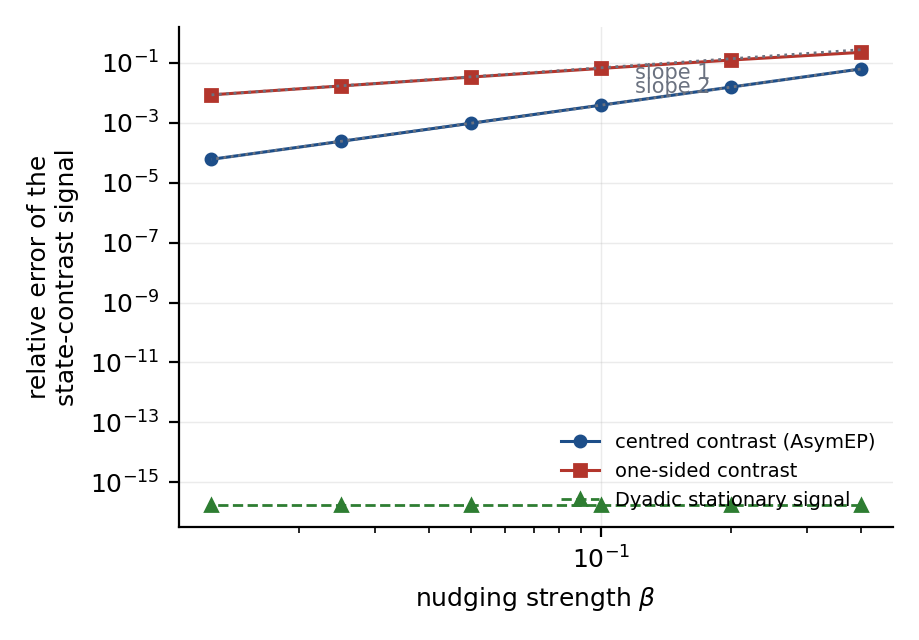
\includegraphics[width=0.62\textwidth]{../assets/fig3_nudge_order.png}
\caption{Relative error of the state-contrast signal against the nudging strength on the
three-state benchmark of Section~\ref{sec:nonnormal}, log-log scale. The centred contrast of the
corrected phase falls with slope $2.002$, the one-sided contrast with slope $0.946$, and the
doubled-state stationary signal sits at machine precision. The fitted orders are produced by the
same run that produces the curves.}
\label{fig:order}
\end{figure}

\subsection{The total budget}

\begin{theorem}[Certified finite-perturbation bound]\label{thm:budget}
Let Assumption~\ref{ass:regular} hold on a neighbourhood $\Omega$ of the branch with
$\sigma_{\min}(A(z)) \ge \alpha > 0$ for $z \in \Omega$, let $\abs{\beta} \le \betamax$ be such
that the perturbation endpoints lie in $\Omega$, and let $(\widehat z^{+\beta}, \widehat z^{-\beta})$
be computed states with certified boxes $X^+$, $X^-$ that contain both the exact roots
$z^{+\beta}, z^{-\beta}$ and the reported candidates $\widehat z^{+\beta}, \widehat z^{-\beta}$,
and, when the states are obtained by
integrating an auxiliary dynamics for time $T$, a certified
finite-time error $\delta_t$. Then
\begin{equation}
\boxed{\
\norm{\widehat g_\beta - d^\star}
\;\le\;
\underbrace{\frac{\norm{B}}{6} M_3 \beta^2}_{E_\beta:\ \text{contrast bias}}
\;+\;
\underbrace{\frac{\norm{B}}{4\betamax}\bigl(\diam X^+ + \diam X^-\bigr)}_{E_z:\ \text{root enclosure}}
\;+\;
\underbrace{\frac{\norm{B}}{\betamax}\delta_t}_{E_t:\ \text{finite time}}
\;+\;
\underbrace{\kappa(A)\, u}_{E_{\mathrm{fp}}:\ \text{rounding}}
\ }
\label{eq:budget}
\end{equation}
with $u$ the unit roundoff and $\kappa(A) = \norm{A}\norm{A^{-1}}$. Each term is either certified
by interval evaluation or explicitly declared as a modelling assumption; none is fitted. The
root-enclosure term follows from the estimator $\widehat g_\beta = B^{\top}(z^{+\beta} -
z^{-\beta})/(2\beta)$ together with $\diam X^\pm = 2 r^\pm$ for boxes of radius $r^\pm$.
\end{theorem}

Theorem~\ref{thm:budget} is the analytic counterpart of Algorithm~\ref{alg:certified}. Four
remarks are in order. First, the budget is stated for $\betamax$, the largest perturbation
strength in the certified domain, so that a single tube certificate covers every candidate below
it. Second, a bound of the form \eqref{eq:budget} is only meaningful when each term is finite on
the certified domain: the contraction certificate below is what makes that true. Third, the
verdict is a comparison of the bound with a tolerance, not a comparison of the observed error
with the tolerance; the latter would be circular, since the observed error is what the certificate
is supposed to bound. Fourth, the four terms are alternatives rather than a checklist that a run
must populate. On the benchmarks of Section~\ref{sec:results} the finite-time term is realised in
a stronger form than the statement requires: instead of bounding an integrator's truncation error,
the endpoint certificate bounds the residual of the returned state and converts it into a distance
to the equilibrium through the certified contraction rate, so $E_t$ is replaced by an
$E_z$ computed from that distance, not by an error estimate for the integration. The rounding term
$E_{\mathrm{fp}}$ is absent for a different reason: candidate states are converted to exact binary
rationals and every subsequent operation is exact, so no rounding enters those certificates at all
and $\kappa(A)u$ overstates a contribution that is zero in that arithmetic.

Two routes to a gradient bound are available, and the two benchmarks exercise different routes. When
the exact rational gradient $d^\star$ of Theorem~\ref{thm:implicit} has a closed form, the verdict
uses the direct interval error
\begin{equation}
D(\beta) = [\underline d,\ \overline d] \supseteq \widehat g_\beta,
\qquad
E(\beta) = \max\bigl\{\abs{\underline d - d^\star},\ \abs{\overline d - d^\star}\bigr\},
\label{eq:errdef}
\end{equation}
so that $\abs{\widehat g_\beta - d^\star} \le E(\beta)$ holds by construction; this is the
quantity reported in Tables~\ref{tab:scan} and~\ref{tab:branch}. It covers both the contrast bias
and the enclosure radius of the endpoints, and it requires no Taylor remainder estimate, since the
truth is known exactly. It is nevertheless a statement about the estimator at one parameter point
rather than a model-independent guarantee, because it presupposes the closed-form truth; that is
precisely why it is used only on the rational benchmark. The truth-free route is
\eqref{eq:budget}, whose terms are computed by interval evaluation alone: it is the route the
three-state benchmark of Section~\ref{sec:nonnormal} takes, and the route available to a user who
has no closed-form gradient, at the cost of constants that may be conservative by orders of
magnitude.

\subsection{Branch-existence certificates and the fail-closed rule}

\begin{theorem}[Krawczyk inclusion]\label{thm:krawczyk}
Let $g: \R^n \to \R^n$ be $C^1$ on a box $X$, let $x \in X$, let $P$ be a nonsingular
$n\times n$ matrix, and let $D g(X)$ be an interval enclosure of the Jacobian on $X$. Define
\begin{equation}
K(X) = x - P\,g(x) + \bigl(I - P\,Dg(X)\bigr)(X - x).
\label{eq:krawczyk}
\end{equation}
If $K(X) \subset \operatorname{int}(X)$ and $\norm{I - P\,Dg(X)}_{\infty} < 1$, then $g$ has
exactly one zero in $X$, and the preconditioned fixed-point map is a contraction on $X$.
\end{theorem}

\begin{corollary}[Uniform certification over a parameter interval]
\label{cor:tube}
Let $g(z,\beta)$ depend on a parameter $\beta \in \mathcal{B}$ and suppose that for the same
box $X$ and preconditioner $P$ the inclusion $K(X,\mathcal{B}) \subset \operatorname{int}(X)$
holds with an interval Jacobian evaluated over both $X$ and $\mathcal{B}$, and that
$\sup_{\beta \in \mathcal{B}}\norm{I - P D_z g(X,\beta)}_{\infty} = c < 1$. Then for every fixed
$\beta \in \mathcal{B}$ there is exactly one root in $X$. If in addition the trace and determinant
of the learning-phase Jacobian $D_z g$ are sign-definite on $X \times \mathcal{B}$ (negative trace,
positive determinant in the two-dimensional case), that root is locally asymptotically stable as a
state of the learning-phase dynamics. Stability of the free equilibrium is a separate property,
governed by $A = D_z F$ and certified separately.
\end{corollary}

Corollary~\ref{cor:tube} is the reason a certification run can cover a continuum of nudging
strengths rather than a single value, and it is the device that lets a controller search over
candidate strengths without re-certifying existence. Branch identity is then a consequence of
geometry rather than of the solver's initial guess: a box whose solution set is certified unique
cannot contain two distinct equilibria, so a deliberately wide box spanning several equilibria
must be rejected by the inclusion test. That rejection is itself part of the acceptance suite.
Containment carries the same argument one level further. Since the box holds exactly one root for
each $\beta$, an endpoint verified to lie inside the tube box lies on the same branch as the free
equilibrium, and the two endpoints of a centred contrast belong to one branch rather than to two.
Without that containment check the two certified endpoints could sit on two different branches and
their difference quotient would be meaningless, which is the failure mode the final rejection rule
of Algorithm~\ref{alg:certified} detects.

\begin{theorem}[Local uniqueness is all that is claimed]\label{thm:local}
The conclusion of Theorem~\ref{thm:krawczyk} and Corollary~\ref{cor:tube} is local: it asserts
existence and uniqueness in the certified box, and no global statement about the number of
equilibria or about convergence of trajectories. Consequently a certificate can be produced for
one branch while another branch, equally stable, is not certified in the same run; and the
presence of an uncertified branch is not evidence against the certified one. The framework is
sound but not complete: a failed inclusion says that the box was too wide for the test, not that
no root is there, so a rejection is a statement about the certificate and never a claim about the
system.
\end{theorem}

\subsection{Non-normality: finite-time bounds are not spectral bounds}

\begin{theorem}[Transient amplification]\label{thm:nonnormal}
Let $A_K = \begin{pmatrix} -1 & K \\ 0 & -1 \end{pmatrix}$ with $K \ge 0$. All eigenvalues equal
$-1$, so the spectral abscissa is $-1$ for every $K$, yet
\begin{equation}
\norm{e^{A_K^{\top} t}}_2 = e^{-t}\,\sqrt{1 + \tfrac{K^2 t^2}{2} + \tfrac{K t}{2}\sqrt{K^2t^2 + 4}}
\label{eq:gain}
\end{equation}
which grows before it decays. Two families appear below and should not be conflated. The closed
form \eqref{eq:gain} is for the equal-eigenvalue case, whose two eigenvalues are both $-1$; it is
the family used for the counterexample of Section~\ref{sec:nonnormal}. The scanned family
$A_K = \begin{pmatrix} -1 & K \\ 0 & -0.1 \end{pmatrix}$, with eigenvalues $-1$ and $-0.1$, has no
equally compact form and is evaluated numerically; the same phenomenon appears there, with the
semigroup norm reaching $15.5$ at $K = 20$. In both families the Lyapunov envelope
$\norm{e^{A^{\top}t}}_2 \le \sqrt{\kappa(P)}\,e^{-\lambda t}$ with
$A P + P A^{\top} = -I$ and $\lambda = 1/(2\norm{P})$ remains valid, but it is not tight: on the
scanned family it stays above the directional adjoint error by four orders of magnitude while
never being violated, and the direct operator-norm bound is itself three orders above the error.
Therefore the finite-time term $E_t$ of Theorem~\ref{thm:budget} must be derived from a semigroup
bound or a certified integrator estimate, not from the spectrum, and a stability certificate for
the equilibrium does not by itself justify a finite-time error bound.
\end{theorem}

\begin{algorithm}[t]
\caption{Certified finite-perturbation gradient update (fail-closed)}
\label{alg:certified}
\begin{enumerate}
\item \textbf{Free equilibrium.} Obtain a candidate $z^{(0)}$ by Newton iteration on
$F(z,\theta)=0$; build a rational box $X^\star$ around the exact rational conversion of
$z^{(0)}$; evaluate \eqref{eq:krawczyk} for $g = F$. If the inclusion fails, halve the box and
retry up to a fixed budget; if it still fails, \textsc{reject}.
\item \textbf{Branch tube.} For the candidate strength $\betamax$, build the corrected learning
field $g(z,\beta) = F(z,\theta) - 2A_{\mathrm a}(z-z^\star) - \beta \grad_z C(z,\theta)$ and
certify $K(X,\mathcal{B}) \subset \operatorname{int}(X)$ over the parameter interval
$\mathcal{B} = [-\betamax, \betamax]$ with the contraction factor of
Corollary~\ref{cor:tube}; certify the Hurwitz signs of the learning Jacobian on the same box.
\item \textbf{Endpoints.} For each of $\pm\beta$, run a floating-point root solve, convert the
returned coordinates to exact binary rationals, build a small rational box and certify it by
Theorem~\ref{thm:krawczyk}. Check that both endpoint boxes lie inside the certified tube box;
otherwise \textsc{reject}, since the two states are then not certified to belong to the same
branch.
\item \textbf{Gradient enclosure.} Form the interval
$D = (X^{+} - X^{-})/(2\beta)$ and the error bound
$E(\beta) = \max\{\abs{\underline d - d^\star}, \abs{\overline d - d^\star}\}$ where $\underline d,
\overline d$ are its endpoints and $d^\star$ is the exact rational implicit gradient
(Theorem~\ref{thm:implicit}); in the absence of a closed-form $d^\star$, use
\eqref{eq:budget}.
\item \textbf{Verdict.} If all certificates pass and $E(\beta) \le \varepsilon$, return the
interval $[\underline d,\overline d]$ with its certificate. Otherwise move to the next candidate
$\beta$ in descending order; if no candidate passes, \textsc{reject} and report which
obligation failed.
\end{enumerate}
\end{algorithm}

\section{Numerical verification}\label{sec:results}

Every number below is produced by the accompanying package. The package runs nine stages and an
automated test suite; a single command reproduces all tables, figures and certificates, and each
stage exits non-zero if one of its assertions fails. Certificates that are accepted were produced
by exact rational interval arithmetic over \texttt{fractions.Fraction}; floating-point root
finders supply candidates only.

\subsection{An exactly solvable non-conservative system with two stable branches}
\label{sec:multistable}

Take
\begin{equation}
F(x,y;\theta) = \begin{pmatrix} x - x^3 + \tfrac15 y + \theta \\[2pt]
-y + \tfrac{1}{10}(x - x^3) \end{pmatrix},
\qquad
C(x,y) = \tfrac12\Bigl[\bigl(x-\tfrac{3}{10}\bigr)^2 + \bigl(y+\tfrac15\bigr)^2\Bigr],
\label{eq:model}
\end{equation}
with $\theta = 0$. The second equation gives $y = (x-x^3)/10$; substituted into the first it
yields $\frac{51}{50}x(1-x^2) = 0$, so the equilibria are exactly
\begin{equation}
z_L = (-1,0), \qquad z_s = (0,0), \qquad z_R = (1,0),
\end{equation}
and the state Jacobian is
\begin{equation}
A(x) = \begin{pmatrix} 1 - 3x^2 & \tfrac15 \\[2pt] \tfrac{1}{10}(1-3x^2) & -1 \end{pmatrix}.
\end{equation}
At $x = \pm 1$ we have $\operatorname{tr}A = -3$ and $\det A = 51/25 > 0$, so both outer
equilibria are locally asymptotically stable; at the origin $\det A = -51/50 < 0$, so it is a
saddle. The two off-diagonal entries are $1/5$ and $-1/5$, so $A$ is not symmetric: the benchmark
is non-conservative and multistable at the same time, and the global uniqueness of equilibria
required by conservative arguments fails (Figure~\ref{fig:phase}). The parameter enters only the
first equation additively, hence $B = (1,0)^{\top}$, and the exact negative gradients are
\begin{equation}
d^\star(z_R) = -\frac{11}{34} \approx -0.3235294118, \qquad
d^\star(z_L) = \frac{67}{102} \approx 0.6568627451 ,
\label{eq:exact-grads}
\end{equation}
computed from Theorem~\ref{thm:implicit} in rational arithmetic, not estimated by finite
differences.

\begin{figure}[t]
\centering
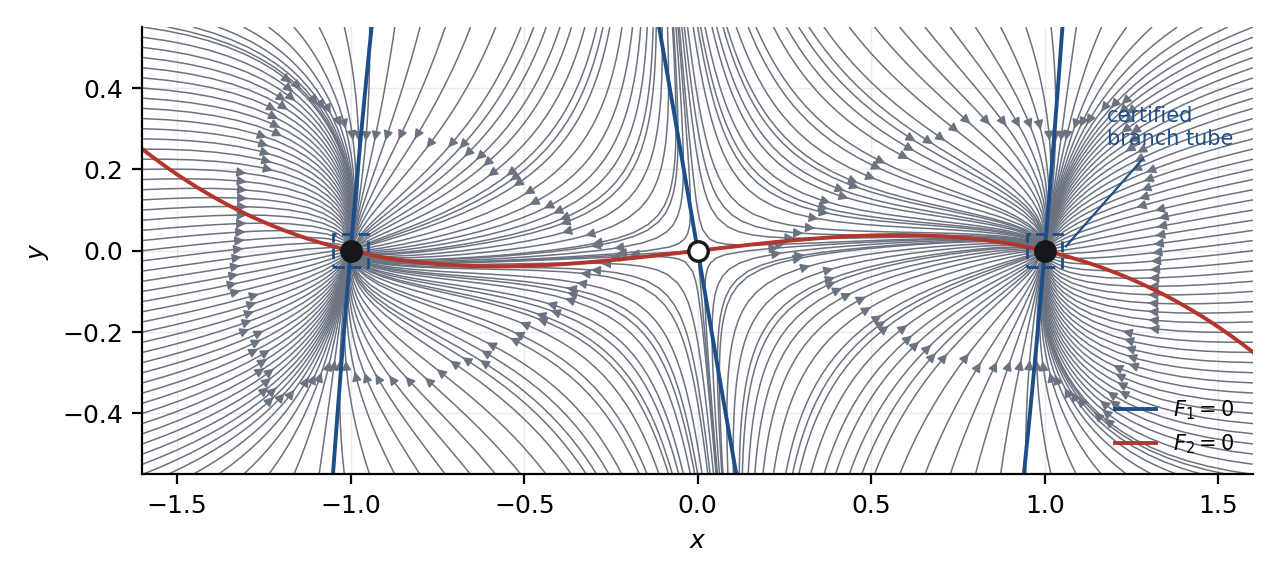
\includegraphics[width=0.86\textwidth]{../assets/fig1_benchmark.png}
\caption{The benchmark \eqref{eq:model}. Nullclines $F_1 = 0$ and $F_2 = 0$, the flow field,
and the three equilibria (filled: stable, open: saddle). Dashed rectangles are the branch tubes
certified in Section~\ref{sec:multistable}: the Krawczyk inclusion holds uniformly for every
$\beta \in [-0.02,0.02]$ on both tubes.}
\label{fig:phase}
\end{figure}

\paragraph{Branch tubes.}
For each stable branch we take the box $X_s = [s-0.05, s+0.05] \times [-0.04, 0.04]$ and the
parameter interval $\mathcal{B} = [-0.02,0.02]$, and evaluate the parametric Krawczyk operator
\eqref{eq:krawczyk} in exact rational arithmetic with the preconditioner
$P = \bigl(D_z g(z_s,0)\bigr)^{-1} = \bigl(A_s^{\top}\bigr)^{-1} = A_s^{-\top}$. Both tubes pass the strict inclusion
test with the same certified contraction factor
\begin{equation}
\sup_{\beta \in \mathcal{B}} \norm{I - P\,D_z g(X_s,\beta)}_{\infty} = \frac{2249}{13600}
\approx 0.165368 < 1 ,
\end{equation}
so by Corollary~\ref{cor:tube} each tube contains exactly one learning-phase root for every
$\beta$ in the interval. On the same tube the learning Jacobian satisfies
\begin{equation}
\operatorname{tr} D_z g \in \Bigl[-\tfrac{1339}{400}, -\tfrac{1067}{400}\Bigr] = [-3.3475,-2.6675],
\qquad
\det D_z g \in \Bigl[\tfrac{4219}{2500}, \tfrac{24199}{10000}\Bigr] = [1.6876,2.4199],
\end{equation}
so the Hurwitz criterion holds throughout the tube: every learning-phase root in it is locally
asymptotically stable as a state of the augmented dynamics, which is what the certificate
establishes. Stability of the free equilibria is the separate statement of
Section~\ref{sec:multistable}, $\operatorname{tr}A = -3$ and $\det A = 51/25 > 0$, and it is a
property of $A = D_z F$ rather than of $D_z g$. Both facts are statements about a continuum of
nudging strengths, not about the one value finally selected.

\paragraph{Nudging selection.}
The controller evaluates candidates in descending order and accepts the first one whose entire
obligation list passes: tube certificate, both endpoint certificates, endpoint containment in the
tube, and the interval error bound against the exact gradient of \eqref{eq:exact-grads} below
tolerance $\varepsilon = 10^{-5}$. Table~\ref{tab:scan} gives the outcome for a dense grid.

\begin{table}[t]
\centering
\small
\caption{Certified worst-branch gradient error bound against the nudging strength on the
benchmark \eqref{eq:model}, tolerance $\varepsilon = 10^{-5}$. Every row is the maximum over the
two stable branches of the interval error \eqref{eq:errdef}. The bias scales as $\beta^2$, and adding the
$1/\beta$ enclosure term gives ratios for successive halvings from $0.02$ of $4.0009$, $3.9912$ and
$3.9271$, bending below $4$ as the enclosure term becomes comparable to the bias. Acceptance stops between
$0.0075$ and $0.005$.}
\label{tab:scan}
\begin{tabular}{rrrl}
\toprule
$\beta$ & worst-branch error bound & branch bounds $(-1,0)$ / $(1,0)$ & decision \\
\midrule
$0.02000$ & $1.2019\times10^{-4}$ & $1.2019\times10^{-4}$ / $1.2588\times10^{-5}$ & rejected, exceeds tolerance \\
$0.01500$ & $6.7593\times10^{-5}$ & $6.7593\times10^{-5}$ / $7.0815\times10^{-6}$ & rejected, exceeds tolerance \\
$0.01250$ & $4.6938\times10^{-5}$ & $4.6938\times10^{-5}$ / $4.9174\times10^{-6}$ & rejected, exceeds tolerance \\
$0.01000$ & $3.0042\times10^{-5}$ & $3.0042\times10^{-5}$ / $3.1473\times10^{-6}$ & rejected, exceeds tolerance \\
$0.00750$ & $1.6905\times10^{-5}$ & $1.6905\times10^{-5}$ / $1.7708\times10^{-6}$ & rejected, exceeds tolerance \\
$\mathbf{0.00500}$ & $\mathbf{7.5271\times10^{-6}}$ & $7.5271\times10^{-6}$ / $7.8826\times10^{-7}$ & \textbf{accepted} \\
$0.00400$ & $4.8295\times10^{-6}$ & $4.8295\times10^{-6}$ / $5.0570\times10^{-7}$ & accepted \\
$0.00250$ & $1.9167\times10^{-6}$ & $1.9167\times10^{-6}$ / $2.0069\times10^{-7}$ & accepted \\
$0.00125$ & $5.4918\times10^{-7}$ & $5.4918\times10^{-7}$ / $5.7493\times10^{-8}$ & accepted \\
$0.00100$ & $4.0027\times10^{-7}$ & $4.0027\times10^{-7}$ / $4.1899\times10^{-8}$ & accepted \\
\bottomrule
\end{tabular}
\end{table}

The selected strength is $\betamax = 0.005$, the largest tested candidate whose bound is below
tolerance. This is not a claim of optimality: it is the largest accepted element of the tested
set under the stated certificates. Table~\ref{tab:branch} reports the branch-level outcome at the
selected strength.

\begin{table}[t]
\centering
\small
\caption{Branch-level certificates at $\beta = 0.005$. The interval column is the certified
enclosure of the centred finite difference \eqref{eq:contrast}; the error bound is
\eqref{eq:errdef} against the exact rational gradient; the observed error is the floating-point
finite difference evaluated at the returned interior point. All four endpoint boxes are certified
by Theorem~\ref{thm:krawczyk} and lie strictly inside the certified tube boxes.}
\label{tab:branch}
\begin{tabular}{lrrrr}
\toprule
Stable branch & exact $d^\star$ & certified difference interval & certified bound & observed error \\
\midrule
$(-1,0)$ & $67/102 = 0.6568627451$ & $[0.6568702322,\ 0.6568702722]$ & $7.5271\times10^{-6}$ & $7.5071\times10^{-6}$ \\
$(1,0)$  & $-11/34 = -0.3235294118$ & $[-0.3235286635,\ -0.3235286235]$ & $7.8826\times10^{-7}$ & $7.6826\times10^{-7}$ \\
\bottomrule
\end{tabular}
\end{table}

Three properties of Table~\ref{tab:branch} should be recorded. The exact gradient lies outside both
difference intervals, because the finite-nudge estimator is biased: the certificate is an
enclosure of the estimator, and the bound then measures the estimator against the truth. The
interval enclosure is tiny (width $4\times10^{-8}$) because the endpoint boxes were certified at
radius $10^{-10}$; the bound is dominated by the bias, not by root uncertainty. Finally, the
observed floating-point error is close to but smaller than the bound, as it must be.

\begin{figure}[t]
\centering
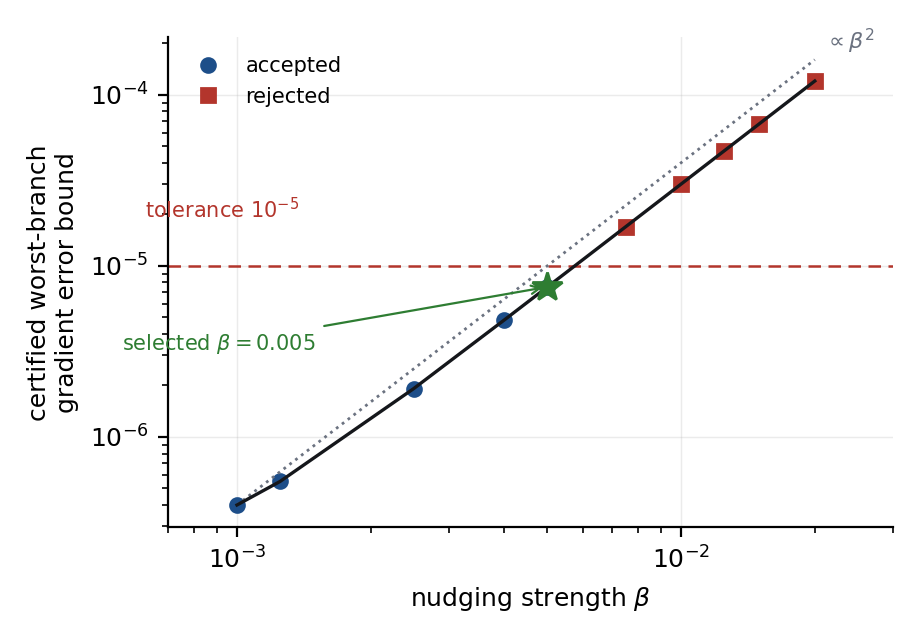
\includegraphics[width=0.52\textwidth]{../assets/fig2_beta_scan.png}
\caption{Certified worst-branch error bound (Table~\ref{tab:scan}) against the nudging strength,
log-log scale. Squares are rejected candidates, circles accepted ones, the star marks the
selected $\betamax = 0.005$, and the dotted line is the quadratic reference. The vertical gap
between the curve and the tolerance line is what the certificate contributes: the decision is
made on the bound, not on an observed error.}
\label{fig:scan}
\end{figure}

\paragraph{Rejection is part of the result.}
Two rejection paths are exercised in the same run. A deliberately wide box
$[-1.2,1.2]\times[-0.1,0.1]$, which contains all three exact equilibria, fails the inclusion test
with contraction factor $183/50 = 3.66 > 1$: the certificate refuses to report a unique root,
which is the correct behaviour for a set containing three of them. Requests outside the certified
parameter domain, for instance $\beta = 0.1$, raise a domain error rather than returning a weaker
bound, so a tolerance cannot be met by silently leaving the certified region. Finally, an
independent high-precision root computation (70 decimal digits) is verified to fall inside each
certified endpoint box; it serves as a cross-check and carries no part of the guarantee, which
comes from the interval inclusion.

\subsection{A three-state non-normal benchmark}\label{sec:nonnormal}

The second benchmark is a smooth, three-state, strongly non-normal system with a closed-form
equilibrium branch,
\begin{equation}
F(z,\theta) = A_0\bigl(z - z^\star(\theta)\bigr) + \gamma \tanh\bigl(K(z - z^\star(\theta))\bigr),
\qquad z^\star(\theta) = L\theta + o,
\label{eq:three-state}
\end{equation}
with
\begin{equation}
A_0 = \begin{pmatrix} -2 & 1.2 & -0.4 \\ -0.3 & -1.8 & 0.5 \\ 0.2 & -0.7 & -1.5 \end{pmatrix},
\quad
K = \begin{pmatrix} 0 & 0.5 & 0.1 \\ -0.2 & 0 & 0.3 \\ 0.1 & -0.4 & 0 \end{pmatrix},
\quad
L = \begin{pmatrix} 1 & 0.2 \\ -0.4 & 0.7 \\ 0.3 & -0.5 \end{pmatrix},
\end{equation}
$\gamma = 0.25$, $o = (0.1,-0.2,0.05)$, $\theta^\star = (0.2,-0.15)$, so that
$z^\star = (0.27,-0.385,0.185)$; the loss is
$C(x) = \tfrac12 (x-t)^{\top}Q(x-t) + c\sum_i(1-\cos x_i)$ with
$Q = \diag(1,1.4,0.8)$, $c = 0.1$ and $t = (0.5,-0.1,0.3)$. The equilibrium Jacobian is
$A = A_0 + \gamma K$ with eigenvalues $-1.8097 \pm 0.9749\,\mathrm i$ and $-1.6805$; despite being
Hurwitz, $A$ is far from normal, which makes this benchmark informative (Section~\ref{sec:budget}
and Theorem~\ref{thm:nonnormal}).

\paragraph{Verification of the gradient identities.}
The implicit gradient of Theorem~\ref{thm:implicit} agrees with a central finite difference of the
objective to a relative error of $6.6\times10^{-11}$, and with reverse-mode automatic
differentiation of the objective to $1.8\times10^{-16}$; the doubled-state stationary identity of
Theorem~\ref{thm:dyadic} reproduces the same direction to $1.8\times10^{-16}$. The uncorrected
vector-field rule \eqref{eq:vf} has relative error $1.55$ on this benchmark, that is, it is not
approximately right at all. The centred contrast of the corrected phase converges with observed
log-log order $2.002$ (one-sided: $0.946$), as predicted by Theorem~\ref{thm:secondorder}; the
doubled-state signal is exact in algebra and limited only by the linear solve
(Figure~\ref{fig:order}).

\paragraph{Certified residual run.}
The exact rational implementation certifies the following constants on the certified domain
$\abs{\beta} \le 0.32$: one-sided contraction rate $\alpha = 0.64$; parameter Jacobian bound
$\norm{B}_F \le 3.24$; $\norm{q(x_0)} \le 0.488$; loss-gradient Lipschitz constant $L_q \le 1.5$;
force derivative bounds $M_2 \le 0.066$, $M_3 \le 0.080$. None of these is fitted or assumed: each
is an assertion in exact rational arithmetic that the code re-evaluates and that raises if
violated. The contraction rate comes from a Gershgorin row-sum bound on the Jacobian of the
learning field, computed over an exact interval enclosure of the state and compared with the
claimed $-0.64$; the parameter-Jacobian bound from an exact Frobenius sum, checked against
$3.24$; the loss-gradient bound from an interval evaluation of $q$ on the certified box; and the
derivative bounds $M_2, M_3$ from the product structure of the force, with the row norms of $K$
themselves bounded by rational constants. From these, the derivative bounds of
Theorem~\ref{thm:secondorder} are computed by implicit differentiation and evaluated at
$\beta = 0.005$ as
\begin{equation}
x_1 \le 0.7714, \qquad x_2 \le 3.6779, \qquad x_3 \le 27.0817,
\qquad E_\beta = \frac{\norm{B}\,\beta^2 x_3}{6} = 3.656\times10^{-4}.
\label{eq:x123}
\end{equation}
The two perturbation endpoints are integrated with a high-accuracy solver and then re-evaluated in
exact rational arithmetic: their residual infinities are bounded by $7.04\times10^{-8}$ and
$7.48\times10^{-8}$, which yields certified distances to the equilibrium of
$1.10\times10^{-7}$ and $1.17\times10^{-7}$ and a solve contribution
$E_z = \norm{B}(r^+ + r^-)/(2\beta) = 3.24 \times (1.0999\times10^{-7} + 1.1688\times10^{-7})/(2\times 0.005) = 7.351\times10^{-5}$,
the enclosure term of \eqref{eq:budget} in its radius form
(Table~\ref{tab:budget}). The total certified bound is $4.391\times10^{-4}$ at tolerance
$5\times10^{-4}$, while the observed gradient error at the same settings is
$1.076\times10^{-5}$: the certificate is $41$ times more conservative than the observed error, and it bounds
it.

\begin{table}[t]
\centering
\small
\caption{Certified budget on the three-state benchmark at $\beta = 0.005$ and integration horizon
$T = 6.0$. The middle column records the value at the shorter horizon $T = 4.0$ that the
controller first tried: the solve term then exceeds the tolerance, so the certificate forces a
longer horizon rather than a relaxed tolerance. All quantities are produced by
\texttt{certified\_gep.py} in exact rational arithmetic where marked certified.}
\label{tab:budget}
\begin{tabular}{lrr}
\toprule
Term & $T = 4.0$ & $T = 6.0$ (selected) \\
\midrule
endpoint residual, $+$ and $-$ & $3.12\times10^{-6}$, $3.26\times10^{-6}$ & $7.04\times10^{-8}$, $7.48\times10^{-8}$ \\
distance to equilibrium, $+$ and $-$ (certified) & $1.10\times10^{-7}$, $1.17\times10^{-7}$ & $1.10\times10^{-7}$, $1.17\times10^{-7}$ \\
contrast bias $E_\beta$ (certified) & $3.656\times10^{-4}$ & $3.656\times10^{-4}$ \\
solver term $E_z$ (certified) & $3.233\times10^{-3}$ & $7.351\times10^{-5}$ \\
total certified bound & $3.599\times10^{-3}$ & $4.391\times10^{-4}$ \\
tolerance & $5\times10^{-4}$ & $5\times10^{-4}$ \\
verdict & rejected & accepted \\
\bottomrule
\end{tabular}
\end{table}

\paragraph{Adaptive controller and integrator comparison.}
An independent adaptive controller selects $(\beta,T,h)$ from the budget alone, without access to
the true gradient: it seeds $T$ from the exact matrix-exponential directional tail, extends it
until both the tail and the observed finite-$\beta$ change pass their thresholds, and scores
candidate nudging strengths by a combined indicator. It selects $\beta = 0.04$, $T = 7.078$, with
a combined indicator of $5.995\times10^{-4}$ made up of a contrast estimate
$1.932\times10^{-4}$, a finite-time change $2.251\times10^{-5}$, a numerical indicator
$1.597\times10^{-5}$ and a state-uncertainty bound $3.679\times10^{-4}$ for a per-phase
uncertainty budget of $5\times10^{-6}$. Its realised direction differs from the exact gradient by
$1.938\times10^{-4}$ in absolute terms ($6.18\times10^{-4}$ relative), and the adjacent-scale
comparison gives an observed order of $2.0006$, consistent with Theorem~\ref{thm:secondorder}. The
same run compares integrators at the selected settings (Table~\ref{tab:integrator}) and performs a
$500$-trial bounded state-noise stress test, in which the triangle inequality combining the noise-free
error and the noise-induced term holds in every trial.

\begin{table}[t]
\centering
\small
\caption{Integrator comparison at the settings selected by the adaptive controller
($\beta = 0.04$, $T = 7.078$). DOP853 at tolerance $10^{-12}$ is used as a high-accuracy
reference; its evaluation count is an internal output-interval count rather than a directly
comparable right-hand-side call count, and it is therefore reported only to indicate order of
magnitude.}
\label{tab:integrator}
\begin{tabular}{lrrr}
\toprule
Integrator & right-hand-side evaluations & accepted steps & gradient error vs reference \\
\midrule
adaptive RK4 (step doubling) & $168$ & $14$ & $7.88\times10^{-7}$ \\
fixed RK4, $h = 0.05$ & $1136$ & $284$ & $2.57\times10^{-11}$ \\
DOP853, tolerance $10^{-12}$ & $8500$ & $708$ & reference \\
\bottomrule
\end{tabular}
\end{table}

\begin{figure}[t]
\centering
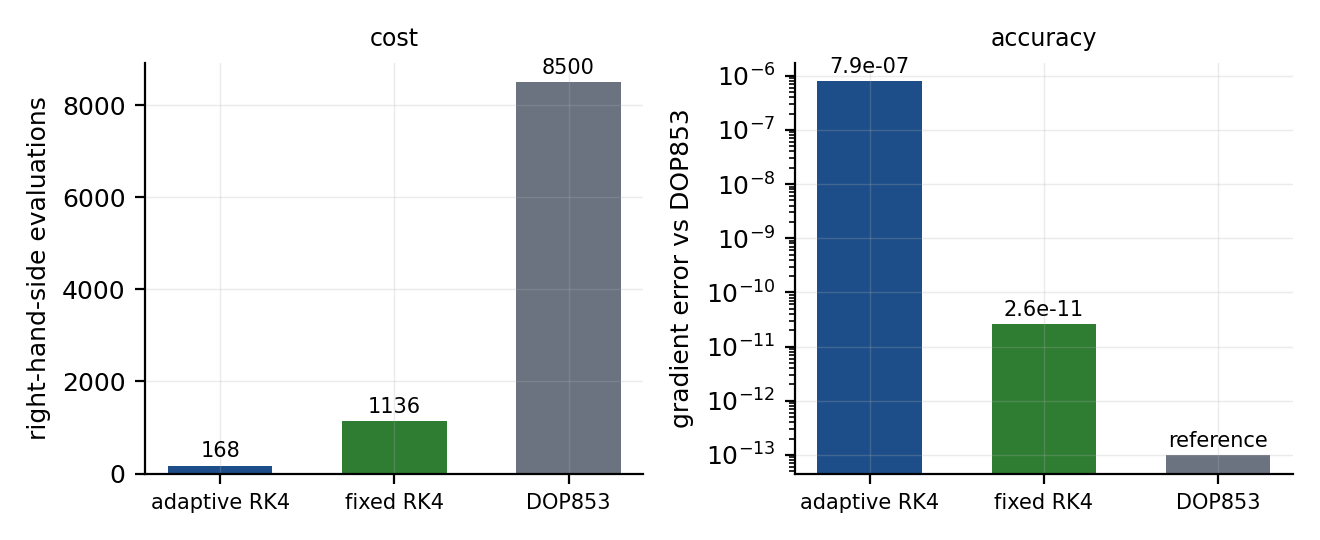
\includegraphics[width=0.78\textwidth]{../assets/fig6_integrators.png}
\caption{Cost and accuracy of the three integrators at the selected settings. The adaptive
scheme reaches $7.9\times10^{-7}$ gradient accuracy with $168$ evaluations, two orders of
magnitude fewer than the high-accuracy reference; the fixed-step scheme spends $1136$ evaluations
to gain four further digits. Neither number enters a certificate: they describe the floating-point
tier of evidence.}
\label{fig:integrators}
\end{figure}

\begin{figure}[t]
\centering
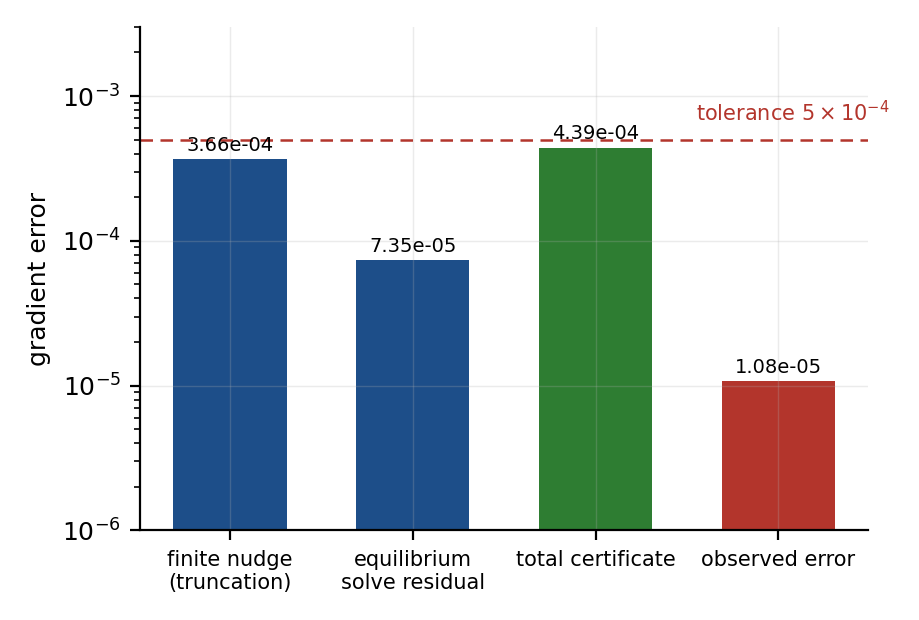
\includegraphics[width=0.58\textwidth]{../assets/fig4_error_budget.png}
\caption{The certified budget of Table~\ref{tab:budget} at $T = 6.0$, with the observed error for
comparison. The certificate is dominated by the contrast bias and is $41$ times larger than the
observed error, which is the intended direction: a bound tighter than the observed error would be
an error, not a certificate.}
\label{fig:budget}
\end{figure}

\subsection{Baselines from the same run}

Table~\ref{tab:levels} already compares the methods on the multistable benchmark. The doubled-state
certificate of Theorem~\ref{thm:residual} is exercised in two ways. First, with an assumed residual
bound $\norm{r_d}_{\infty} \le 10^{-10}$ and the exact constant $\norm{A^{-\top}}_{\infty} = 55/51$,
the bound \eqref{eq:residual} evaluates to $11/10200000000 = 1.0784\times10^{-9}$ at
$\beta = 0.1$ and to $11/10200000 = 1.0784\times10^{-6}$ at $\beta = 10^{-4}$, growing as
$1/\abs{\beta}$: the same amplification mechanism as in the budget. Second, and more stringently,
the float64 linear solve that produces $\widehat d$ is re-evaluated in exact rational arithmetic:
each returned coordinate is read as its exact binary rational value, the residual
$r_d = A^{\top}\widehat d - \beta q$ is recomputed with rational arithmetic, and the resulting
bound covers the observed error in all four cases (Table~\ref{tab:dyadic}). This replaces the
residual from an assumption to a measurement, while remaining a statement about a linear
subproblem with an exactly known midpoint.

\begin{table}[t]
\centering
\small
\caption{Exact rational re-evaluation of the float64 difference solve on the benchmark
\eqref{eq:model}, branch $(1,0)$. The residual is recomputed from the exact binary rational values
of the returned coordinates; the bound is \eqref{eq:residual} with
$\norm{A^{-\top}}_{\infty} = 55/51$; the observed error is the distance of $\widehat d/\beta$ from
the exact gradient $-11/34$.}
\label{tab:dyadic}
\begin{tabular}{rrrr}
\toprule
$\beta$ & exact residual $\norm{r_d}_\infty$ & certified bound & observed error \\
\midrule
$0.1$ & $1.110\times10^{-17}$ & $1.1973\times10^{-16}$ & $5.7144\times10^{-17}$ \\
$0.01$ & $9.541\times10^{-19}$ & $1.0289\times10^{-16}$ & $4.5919\times10^{-17}$ \\
$0.001$ & $6.505\times10^{-20}$ & $7.0154\times10^{-17}$ & $3.5077\times10^{-17}$ \\
$0.0001$ & $8.809\times10^{-21}$ & $9.5001\times10^{-17}$ & $4.3846\times10^{-17}$ \\
\bottomrule
\end{tabular}
\end{table}

\subsection{Non-normality inflates finite-time bounds but not the error}
\label{sec:nonnormal}

The family $A_K = \begin{pmatrix} -1 & K \\ 0 & -0.1 \end{pmatrix}$ has fixed eigenvalues
$-1$ and $-0.1$ and increasing non-normality measured by the logarithmic norm
$\mu_2(A_K) = \tfrac12\lambda_{\max}(A_K + A_K^{\top})$ and by $\kappa_2(A_K)$. The first-order
finite-time adjoint tail is $A^{-\top}e^{A^{\top}t}q$ with $q$ chosen, adversarially, as the
right singular vector of $A^{-\top}$ associated with its smallest singular value, so that the
initial tail is small and can grow.

\begin{table}[t]
\centering
\small
\caption{Transient behaviour of the adjoint response on the family $A_K$. The two eigenvalues are
$-1$ and $-0.1$ for every row, the spectral abscissa is constant, and yet both the semigroup norm
and the finite-time adjoint error grow by more than an order of magnitude. The last column is the
ratio of the largest finite-time gradient error to its initial value.}
\label{tab:nonnormal}
\begin{tabular}{rrrrrr}
\toprule
$K$ & $\kappa_2(A_K)$ & $\mu_2$ & $\max_t\norm{e^{A_K^{\top}t}}_2$ & time of maximum & gradient error amplification \\
\midrule
$0$ & $10.0$ & $-0.100$ & $1.000$ & $0.00$ & $1.000$ \\
$1$ & $20.05$ & $0.123$ & $1.125$ & $1.66$ & $1.000$ \\
$2$ & $50.08$ & $0.547$ & $1.738$ & $2.30$ & $1.518$ \\
$5$ & $260.10$ & $1.990$ & $3.949$ & $2.51$ & $3.857$ \\
$10$ & $1010.10$ & $4.470$ & $7.782$ & $2.55$ & $7.735$ \\
$20$ & $4010.10$ & $9.460$ & $15.505$ & $2.56$ & $15.481$ \\
\bottomrule
\end{tabular}
\end{table}

The smallest instance is a two-dimensional counterexample, which we state explicitly:
$A = \begin{pmatrix} -1 & 10 \\ 0 & -1 \end{pmatrix}$ with $q = (0,1)^{\top}$ gives
$A^{-1}q = (-10,-1)$ and $A^{-\top}q = (0,-1)$, a relative gap of $10$, while
$\kappa_2(A) = 101.99$ and the semigroup norm peaks at $3.716$ at $t = 0.98$. This instance
belongs to the equal-eigenvalue family of Theorem~\ref{thm:nonnormal} and is not the $K = 10$ row
of Table~\ref{tab:nonnormal}, which has eigenvalues $-1$ and $-0.1$ and hence the larger condition
number $1010.10$. A finite-time
argument based on the eigenvalues would predict monotone decay throughout and would therefore be
in error by an order of magnitude in both the response and its bound.

\begin{figure}[t]
\centering
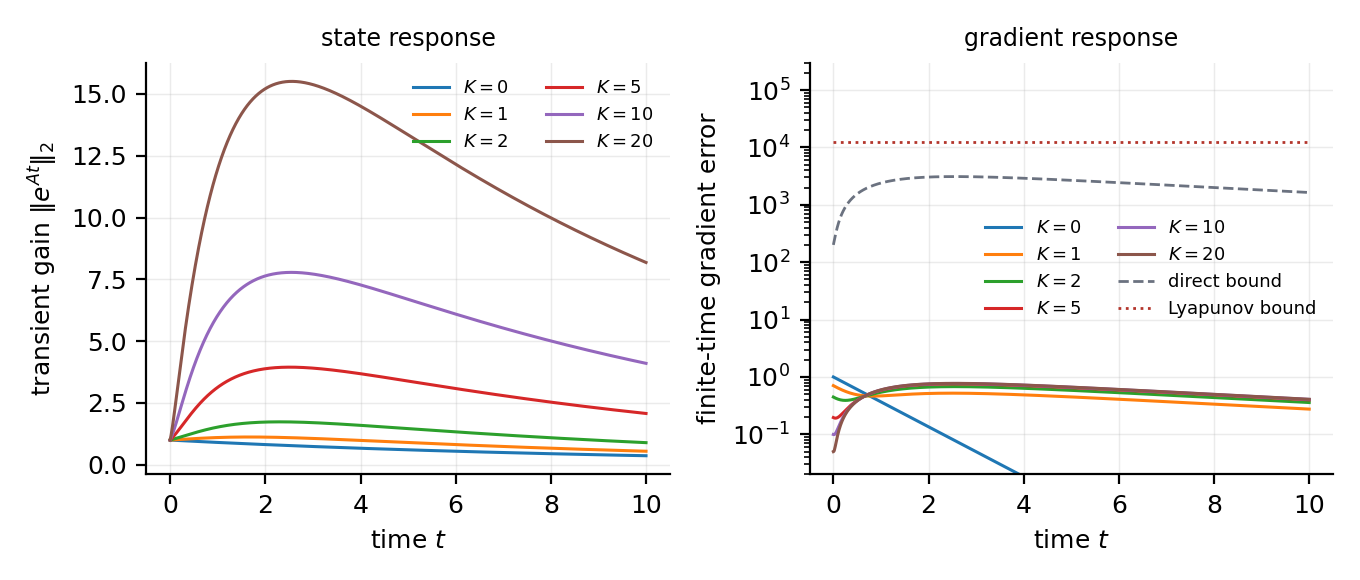
\includegraphics[width=0.92\textwidth]{../assets/fig5_nonnormal.png}
\caption{Left: semigroup norm $\norm{e^{A_K^{\top}t}}_2$ for the family of
Table~\ref{tab:nonnormal}; the eigenvalues are $-1$ and $-0.1$ in every curve. Right: the
finite-time adjoint error $\norm{A^{-\top}e^{A^{\top}t}q}$ (solid), the direct operator-norm bound
(dashed) and the Lyapunov envelope (dotted) for $K = 20$, log scale. The direct bound is valid but
three orders of magnitude loose; the Lyapunov envelope is four. Both are needed as options,
because the direct bound is unavailable when only a Lyapunov function is known, and the envelope
is unusable when sharpness matters.}
\label{fig:nonnormal}
\end{figure}

\subsection{Reproducibility}

The package runs in under a minute on a laptop, with no dependence on precomputed artefacts.
Running the driver executes, in order, the analytic
validation, the bias and trade-off audits, the adaptive controller, the exact rational residual
certificate, the multibranch Krawczyk certificate, the baseline comparison, the two doubled-state
certificate stages and the dense nudging scan, and then the unit test suite; it writes logs and
JSON artefacts and fails if any stage or any of the eight unit tests fails. The unit tests assert
the properties that the paper relies on: two stable branches and one saddle with exact traces and
determinants; passing tube certificates with contraction below one; the selection of
$\beta = 1/200$ with a worst-branch bound below tolerance; containment of endpoint boxes in tubes
and enclosure of the floating-point finite difference; rejection of the wide multibranch box;
containment of 70-digit roots in the certified boxes; fail-closed behaviour outside the certified
domain; and the exact gradient values $67/102$ and $-11/34$.

\section{Discussion}\label{sec:discussion}

\paragraph{What has been certified, and what has not.}
The analytic statements of Sections~\ref{sec:exact}--\ref{sec:budget} are unconditional given
Assumption~\ref{ass:regular}: the gradient identity, the bias criterion, the sensitivity-adjoint
dichotomy, the second-order contrast bound and the residual transfer inequality hold for any
smooth non-conservative system with a regular equilibrium. The numerical certificates are
statements about the two benchmarks, and their conclusions are intervals that contain the exact
rational answer: on the multistable benchmark, both stable branches and both perturbation
endpoints are certified, the parameter tube is certified uniformly over
$\beta \in [-0.02,0.02]$, stability holds throughout the tube, and the update is accepted or
rejected against a tolerance by comparing a certified bound rather than an observed error. What is
not claimed is any statement about trajectories that have not converged, any global count of
equilibria, any performance comparison with backpropagation, or any transfer to systems whose
coefficients are estimated from data.

\paragraph{Relation to finite-nudge exactness in thermal ensembles.}
For Gibbs ensembles the two-phase contrast is exactly the gradient of a free-energy difference at
any finite nudging strength and temperature, and the deterministic rule is recovered in the
zero-temperature limit \cite{litman2026}. Our setting is the deterministic one, and our object is
the gap that remains there: the finite-nudge deficit of the deterministic contrast, bounded in
Theorem~\ref{thm:secondorder} with a computable constant. The two results are complementary rather
than competing. The thermal identity says that finite nudging is not a bias when the ensemble is
sampled correctly; the deterministic analysis says how large the bias is when it is not, and the
certificate says when the resulting estimate may be trusted.

\paragraph{Relation to exact non-conservative algorithms.}
The corrected learning phase and the doubled-state construction are prior work
\cite{scurria2026}, as is the compartmental construction behind dual propagation
\cite{hoier2023}; the bias of the uncorrected rule, and the separation of finite-nudge from
asymmetry bias, are from \cite{laborieux2024,scellier2018}. This paper does not claim any of the
update rules. It contributes the conditions under which their computed output carries a guarantee,
and the numerical machinery that produces one.

\paragraph{The two failure modes that certificates detect.}
Two failure modes escape residual-based reasoning. First, the sensitivity-adjoint gap of
Proposition~\ref{prop:sens}: on the benchmark the uncorrected rule is in error by $12\%$ relative
while its residual is $10^{-17}$, so a small residual certifies nothing about the direction.
Second, non-normality: Table~\ref{tab:nonnormal} shows that eigenvalues fixed at $-1$ and $-0.1$
permit a $15.5$-fold transient amplification of the adjoint response, so a finite-time error bound
must come from a semigroup or integrator certificate and not from stability of the equilibrium.
Both are properties of the model, and both are handled by the budget of
Theorem~\ref{thm:budget}: the first by measuring against the implicit gradient rather than against
the estimator's own fixed point, the second by carrying a genuine finite-time term.

\paragraph{Cost.}
Certification requires interval evaluation of the Jacobian on a box, at cost $O(n^3)$ per
inclusion test for a dense Jacobian, plus exact rational arithmetic whose integers grow with the
number of operations. At the scale of the benchmarks ($n = 2$ and $n = 3$) the entire certified
pipeline runs in well under a second, including both branches, both endpoints, the dense nudging
grid and the wide-box rejection. The practical question for larger systems is not the asymptotic
cost of interval arithmetic but whether the boxes stay tight enough for the inclusion to succeed;
that is an empirical question in a dimension not examined here, and it is the main direction for
future work.

\paragraph{Limitations.}
(i) All statements are local: they concern a certified box around a regular isolated equilibrium,
not global properties of the dynamics. (ii) The regularity requirement $\sigma_{\min}(A) > 0$
excludes bifurcation points and near-singular branches; the framework would have to be extended,
not merely enlarged, to cover them. (iii) The benchmarks are of dimension two and three; cost and
tightness in higher dimension are unmeasured. (iv) Coefficients, the loss and the free equilibrium
are treated as exactly known rational data; measurement noise, parameter intervals and model
mismatch are outside the certificate, and the state-noise stress test only *checks* a triangle
bound rather than certifying it. (v) Certificates cover stationary states and finite-difference
gradients, not validated envelopes of entire trajectories. (vi) The corrector $2A_{\mathrm a}$ is
assumed exactly available, which in hardware would require an estimate; the certificate would then
inherit the estimation error as an additional term. (vii) The proofs have been implemented as
tests over exact rational arithmetic, but they have not been formalised in a proof assistant.

\section{Conclusion}

Equilibrium propagation beyond conservative systems is now supported by exact-gradient algorithms
and by thermal-ensemble exactness results. The output of a run, however, is a pair of numerical
states and a quotient by a small number. This paper has argued that the missing
object is a certificate, and has supplied one: exact gradient conditions for smooth
non-conservative systems with regular equilibria, a finite-perturbation error budget whose
constants are computed rather than fitted, a branch-aware interval certificate that establishes
existence and uniqueness uniformly over a parameter interval, and a fail-closed update rule that
returns an interval or refuses. On an exactly solvable non-conservative system with two stable
branches and a saddle, the pipeline certifies both branches, both perturbation endpoints and the
whole nudging tube in rational arithmetic, accepts $\beta = 0.005$ with a worst-branch bound of
$7.53\times10^{-6}$ at tolerance $10^{-5}$, and rejects both larger nudging strengths and a box
that spans all three equilibria. The two benchmarks support one general observation: in
non-conservative and non-normal systems, neither a small residual nor a stable spectrum implies
that an EP update is what it appears to be, and only a certificate distinguishes the two cases.

\appendix

\section{Proofs}\label{app:proofs}

\begin{proof}[Proof of Theorem~\ref{thm:implicit}]
Differentiating $F(z^\star(\theta),\theta) = 0$ with respect to $\theta$ gives
$A\,D_\theta z^\star + B = 0$, hence $D_\theta z^\star = -A^{-1}B$. Since
$L(\theta) = C(z^\star(\theta),\theta)$, the chain rule gives
$\grad_\theta L = \partial_\theta C + (D_\theta z^\star)^{\top} q
= \partial_\theta C - B^{\top}A^{-\top}q$.
\end{proof}

\begin{proof}[Proof of Proposition~\ref{prop:sens}]
Let $\varphi(\beta)$ denote the root of the uncorrected nudged equation
\eqref{eq:vf} near $z^\star$. Differentiating
$F(\varphi(\beta)) - \beta\grad C(\varphi(\beta)) = 0$ at $\beta = 0$ gives
$A\varphi'(0) - q = 0$, that is $\varphi'(0) = A^{-1}q = s$. The centred difference
$(\varphi(\beta)-\varphi(-\beta))/(2\beta)$ equals $\varphi'(0)$ up to the even-order term
$\tfrac16\varphi'''(0)\beta^2$. The parameter gradient requires
$\lambda = A^{-\top}q$ by Theorem~\ref{thm:implicit}, and $A^{-1} = A^{-\top}$ exactly when
$A = A^{\top}$.
\end{proof}

\begin{proof}[Proof of Theorem~\ref{thm:vf}]
Combining the infinitesimal response $A^{-1}q$ for \eqref{eq:vf} with the contrast
\eqref{eq:contrast} gives $\widehat g_0 = B^{\top}A^{-1}q$, while the true negative gradient is
$B^{\top}A^{-\top}q$; subtracting yields \eqref{eq:vf-bias}. Exactness for a fixed $q$ is
therefore equivalent to $B^{\top}(A^{-1}-A^{-\top})q = 0$, and exactness for all $q$ in a
subspace $S$ is equivalent to \eqref{eq:vf-subspace}. The claim of
Example~\ref{ex:restricted} follows by direct evaluation of the $2\times2$ matrices.
\end{proof}

\begin{proof}[Proof of Theorem~\ref{thm:asym}]
With $g(z,\beta) = F(z) - 2A_{\mathrm a}(z-z^\star) - \beta\grad C(z)$ we have
$D_z g(z^\star,0) = A - 2A_{\mathrm a} = A - (A - A^{\top}) = A^{\top}$. Differentiating
$g(\varphi(\beta),\beta) = 0$ at $\beta = 0$ gives $A^{\top}\varphi'(0) - \grad C(z^\star) = 0$,
hence $\varphi'(0) = A^{-\top}q = \lambda$.
\end{proof}

\begin{proof}[Proof of Theorem~\ref{thm:dyadic}]
By hypothesis the midpoint satisfies $F(m) = 0$ and the difference satisfies
$A(m)^{\top}d = \beta\grad C(m)$; multiplying by $A(m)^{-\top}$ (which exists because $A(m)$ is
nonsingular) gives $d = \beta A(m)^{-\top}\grad C(m)$ for every $\beta \neq 0$. If $m$ is the free
equilibrium and $C$ does not depend explicitly on $\theta$, then
$B^{\top}d/\beta = B^{\top}A^{-\top}q$, which is the true negative gradient of
Theorem~\ref{thm:implicit}.
\end{proof}

\begin{proof}[Proof of Theorem~\ref{thm:residual}]
Substituting the definition of $r_d$ into
$\widehat d/\beta - A(\widehat m)^{-\top}\grad C(\widehat m)$ gives
$\beta^{-1}A(\widehat m)^{-\top}\bigl(A(\widehat m)^{\top}\widehat d - \beta \grad C(\widehat m)\bigr)
= \beta^{-1}A(\widehat m)^{-\top}r_d$, and taking norms yields \eqref{eq:residual}. The constant
$55/51$ is the infinity norm of $\begin{pmatrix} -25/51 & 5/51 \\ -5/51 & -50/51 \end{pmatrix}$,
the exact inverse transpose of $A$ at the benchmark branch, verifiable in rational arithmetic.
\end{proof}

\begin{proof}[Proof of Theorem~\ref{thm:secondorder}]
The map $\beta \mapsto \varphi(\beta)$ is $C^3$ in a neighbourhood of $\beta = 0$ by the implicit
function theorem applied to $(z,\beta) \mapsto g(z,\beta)$ at $(z^\star,0)$, whose Jacobian
$A^{\top}$ is nonsingular by Assumption~\ref{ass:regular}. Write the third-order expansion
$\varphi(\beta) = z^\star + \beta\lambda + \tfrac12\beta^2\varphi''(0) + R(\beta)$ with
$\norm{R(\beta)} \le \tfrac16 M_3\abs{\beta}^3$. Then
$(\varphi(\beta)-\varphi(-\beta))/(2\beta) = \lambda + (R(\beta)-R(-\beta))/(2\beta)$, whose norm
is at most $\tfrac16 M_3\beta^2$ by the triangle inequality and the bound on $R$. Applying
$\widehat g_\beta - d^\star = B^{\top}\bigl((\varphi(\beta)-\varphi(-\beta))/(2\beta) - \lambda\bigr)$
yields \eqref{eq:secondorder-grad}.
\end{proof}

\begin{proof}[Proof of Theorem~\ref{thm:krawczyk}]
Let $\psi(z) = z - P\,g(z)$. For $z \in X$ the mean value theorem gives
$\psi(z) = x - P\,g(x) + \bigl(I - P\,Dg(\xi)\bigr)(z - x)$ for some $\xi$ on the segment from
$x$ to $z$. Since $Dg(\xi)$ lies in the interval enclosure $Dg(X)$, the right-hand side lies in
$K(X)$, so $\psi$ maps $X$ into $\operatorname{int}(X)$ whenever the inclusion holds. In addition
$\norm{D\psi(X)}_{\infty} = \norm{I - P\,Dg(X)}_{\infty} < 1$, so $\psi$ is a contraction on $X$
and has exactly one fixed point there by the Banach fixed-point theorem; fixed points of $\psi$
coincide with zeros of $g$ because $P$ is
nonsingular. The parametric statement of Corollary~\ref{cor:tube} follows by applying the argument
for each fixed $\beta$ with the same box, which the interval evaluation over $\mathcal{B}$ covers
uniformly.
\end{proof}

\begin{proof}[Proof of Theorem~\ref{thm:nonnormal}]
For $A_K = \begin{pmatrix} -1 & K \\ 0 & -1 \end{pmatrix}$ we have
$A_K^{\top} = \begin{pmatrix} -1 & 0 \\ K & -1 \end{pmatrix}$ and
$e^{A_K^{\top}t} = e^{-t}\begin{pmatrix} 1 & 0 \\ Kt & 1 \end{pmatrix}$, so
$\norm{e^{A_K^{\top}t}}_2^2 = e^{-2t}\lambda_{\max}\bigl(\begin{pmatrix} 1+K^2t^2 & Kt \\ Kt & 1\end{pmatrix}\bigr)$,
which yields \eqref{eq:gain} after evaluating the larger eigenvalue. The Lyapunov inequality
$\norm{e^{A^{\top}t}}_2 \le \sqrt{\kappa_2(P)}e^{-\lambda t}$ with $AP + PA^{\top} = -I$ and
$\lambda = 1/(2\norm{P}_2)$ is standard; its looseness on the scanned family is measured in
Table~\ref{tab:nonnormal} and Figure~\ref{fig:nonnormal}.
\end{proof}

\section{Exact rational constants}\label{app:constants}

The following quantities appear in the certificates and are computed in rational arithmetic; the
second column gives the exact fraction, the third its decimal form.

\begin{center}
\small
\begin{tabular}{llr}
\toprule
Quantity & Exact value & Decimal \\
\midrule
true gradient, branch $(-1,0)$ & $67/102$ & $0.6568627451$ \\
true gradient, branch $(1,0)$ & $-11/34$ & $-0.3235294118$ \\
determinant of $A$ at $\pm1$ & $51/25$ & $2.04$ \\
trace of $A$ at $\pm1$ & $-3$ & $-3$ \\
preconditioned contraction, both tubes & $2249/13600$ & $0.1653676471$ \\
trace interval of the learning Jacobian & $[-1339/400,\,-1067/400]$ & $[-3.3475,-2.6675]$ \\
determinant interval of the learning Jacobian & $[4219/2500,\,24199/10000]$ & $[1.6876,2.4199]$ \\
contraction of the rejected wide box & $183/50$ & $3.66$ \\
infinity norm of $A^{-\top}$ on the benchmark & $55/51$ & $1.0784313725$ \\
tolerance & $1/100000$ & $10^{-5}$ \\
\bottomrule
\end{tabular}
\end{center}

\section{Reproducibility}\label{app:repro}

The package contains nine runnable stages and one test module:
\texttt{run\_validation.py} (analytic gradient, finite differences, error decomposition),
\texttt{run\_stage2.py} (task-restricted exactness, nudging trade-off, non-normal transient),
\texttt{run\_stage3.py} (adaptive controller, integrator comparison, tighter non-normal bounds),
\texttt{certified\_gep.py} (exact rational residual certificate on the three-state benchmark),
\texttt{certified\_multibranch\_gep.py} (exact rational multibranch Krawczyk certificate),
\texttt{beta\_scan.py} (dense nudging scan and the data of Figure~\ref{fig:scan}),
\texttt{unified\_baselines.py}, \texttt{dyadic\_residual\_certificate.py} and
\texttt{dyadic\_finite\_precision\_certificate.py} (baselines and the two doubled-state
certificates), plus \texttt{tests/test\_stage5.py} with eight assertions.
\texttt{run\_all.py} executes all of them, writes \texttt{results/} and \texttt{logs/}, runs the
test suite, and exits non-zero on any failure; \texttt{make\_figures.py} regenerates every figure
of this paper from the artefacts. The certificate JSON files carry both decimal and exact
fractional forms of every accepted bound, so a reader can re-verify an accepted claim without
re-running the pipeline.

\begin{thebibliography}{99}
\small

\bibitem{bai2019} S. Bai, J. Z. Kolter, and V. Koltun. Deep equilibrium models. In
\emph{Advances in Neural Information Processing Systems}, 2019.

\bibitem{ernoult2019} M. Ernoult, J. Grollier, D. Querlioz, Y. Bengio, and B. Scellier.
Equivalence of equilibrium propagation and recurrent backpropagation.
\emph{Neural Computation}, 31(2):312--329, 2019.

\bibitem{higham2008} N. J. Higham. \emph{Functions of Matrices: Theory and Computation}.
SIAM, 2008.

\bibitem{hoier2023} R. H{\o}ier, D. Staudt, and C. Zach. Dual propagation: accelerating
contrastive Hebbian learning with dyadic neurons. In \emph{Proceedings of the 40th International
Conference on Machine Learning}, PMLR 202:13141--13156, 2023.

\bibitem{hopfield1984} J. J. Hopfield. Neurons with graded response have collective computational
properties like those of two-state neurons. \emph{Proceedings of the National Academy of
Sciences}, 81(10):3088--3092, 1984.

\bibitem{kendall2020} J. Kendall, R. Pantone, K. Manickavasagam, Y. Bengio, and B. Scellier.
Training end-to-end analog neural networks with equilibrium propagation. arXiv:2006.01981, 2020.

\bibitem{krawczyk1969} R. Krawczyk. Newton-Algorithmen zur Bestimmung von Nullstellen mit
Fehlerschranken. \emph{Computing}, 4:187--201, 1969.

\bibitem{laborieux2024} A. Laborieux and F. Zenke. Improving equilibrium propagation without
weight symmetry through Jacobian homeostasis. In \emph{International Conference on Learning
Representations}, 2024. arXiv:2309.02214.

\bibitem{litman2026} E. Litman. Finite-nudge equilibrium propagation in thermal ensembles.
arXiv:2511.22024v2, 2026.

\bibitem{massar2025} S. Massar and B. M. Mognetti. Equilibrium propagation: the quantum and the
thermal cases. \emph{Quantum Studies: Mathematics and Foundations}, 2025. arXiv:2405.08467.

\bibitem{movellan1991} J. R. Movellan. Contrastive Hebbian learning in the continuous Hopfield
model. In \emph{Connectionist Models: Proceedings of the 1990 Summer School}, 1991.

\bibitem{neumaier1990} A. Neumaier. \emph{Interval Methods for Systems of Equations}. Cambridge
University Press, 1990.

\bibitem{pineda1987} F. J. Pineda. Generalization of back-propagation to recurrent neural
networks. \emph{Physical Review Letters}, 59(19):2229--2232, 1987.

\bibitem{rump2010} S. M. Rump. Verification methods: rigorous results using floating-point
arithmetic. \emph{Acta Numerica}, 19:287--449, 2010.

\bibitem{scellier2017} B. Scellier and Y. Bengio. Equilibrium propagation: bridging the gap
between energy-based models and backpropagation. \emph{Frontiers in Computational Neuroscience},
11:24, 2017.

\bibitem{scellier2018} B. Scellier, A. Goyal, J. Binas, T. Mesnard, and Y. Bengio. Generalization
of equilibrium propagation to vector field dynamics. arXiv:1808.04873, 2018.

\bibitem{scurria2026} A. E. Scurria, D. Vanden Abeele, B. M. Mognetti, and S. Massar. Equilibrium
propagation for non-conservative systems. In \emph{Proceedings of the 43rd International
Conference on Machine Learning}, 2026. arXiv:2602.03670.

\bibitem{trefethen2005} L. N. Trefethen and M. Embree. \emph{Spectra and Pseudospectra: The
Behavior of Nonnormal Matrices and Operators}. Princeton University Press, 2005.

\bibitem{yi2023} S.-i. Yi, J. D. Kendall, R. S. Williams, and S. Kumar. Activity-difference
training of deep neural networks using memristor crossbars. \emph{Nature Electronics}, 6:45--51,
2023.

\end{thebibliography}

\end{document}
